\documentclass[a4paper,12pt]{article}
\usepackage{ecography}
\usepackage{lmodern}
\usepackage{amsmath}
\usepackage{xfrac}
\usepackage{lineno}
\usepackage{color}

\renewcommand{\familydefault}{\sfdefault}

%\nolinenumbers

\title{A Recipe for Scavenging \textcolor{blue}{in Vertebrates} - the natural history of a behaviour}

\running{Scavenging in vertebrates}

\author{Adam Kane, Kevin Healy, Thomas Guillerme, Graeme D. Ruxton, \\ \& Andrew L. Jackson.}

\affiliations{
\item A. Kane (\url{adam.kane@ucc.ie}), University College Cork, Cooperage Building, School of Biological Earth and Environmental Sciences, Cork, Ireland.
\item K. Healy and A.L. Jackson, Trinity College Dublin, Department of Zoology, School of Natural Sciences, Dublin 2, Ireland; Trinity Centre for Biodiversity Research, Trinity College Dublin, Dublin 2, Ireland.
\item T. Guillerme, Imperial College London, Silwood Park Campus, Department of Life Sciences, Buckhurst Road, Ascot SL5 7PY, United Kingdom.
\item G. Ruxton, School of Biology, Sir Harold Mitchell Building, Greenside Place, St Andrews, KY16 9TH, United Kingdom.
}

\nwords{9999}


\begin{document}

\maketitle


\begin{abstract} 
Despite its prevalence, scavenging is a difficult behaviour to observe in modern day carnivores and impossible to study directly in extinct species. 
Yet, there are certain intrinsic and environmental features of a species that push it towards a scavenging lifestyle. 
These can be thought of as some of the principal parameters in optimal foraging theory namely, encounter rate, handling time and prey availability. 
We use these components to highlight the morphologies and environments that would have been conducive to scavenging over geological time by focusing on the dominant vertebrate groups of the land, sea and air. 
The result is a synthesis on the natural history of scavenging. 
These features that make up our \textcolor{blue}{qualitative} scale of scavenging can be applied to any given species and allow us to judge the likely importance of this foraging behaviour.   
\end{abstract}

\newpage


\section{Introduction}

\textcolor{blue}{Historically, food webs have classified most acts of carnivory as predation events \citep{wilson2011scavenging}. 
This is clearly a mistaken view because of the existence of scavenging, a behaviour displayed by almost all carnivorous vertebrates \citep{devault2003scavenging}. 
Recent research has begun to redress this imbalance by recognising the prevalence of scavenging and its implications for trophic ecology across modern ecosystems \citep{pereira2014facultative,periquet2015lion}.
By increasing multichannel feeding and the number of food web links, scavenging can confer stability to an ecosystem \citep{moleon2015living}. 
Indeed, there is no discrete divide between predators and scavengers but rather a continuous gradient in terms of the proportion of carrion in the diet \citep{pereira2014facultative}.
Even vultures, the canonical example of obligate scavengers, can hunt \citep{margalida2011scavenger}. While it is relatively easy to determine whether a species engages in scavenging through observation, determining the proportion of carrion in the diet requires extensive behavioral data. This is because approaches such as stomach content and stable isotope analysis are unable to distinguish between scavenging and predation.} % (I put this in to placate the reviewer who said it was easy).
Unfortunately, the lack of direct behavioural data makes it even more difficult to discern scavenging from predation among extinct forms where it was surely exhibited by prehistoric vertebrate carnivores.
Some simple heuristics can inform us whether or not the prey was scavenged, for instance, in cases where it was simply too large to have been killed by the ostensible predator \citep{pobiner2008paleoecological}.
But clearly, a scavenger does not only feed on dead animals too big for it to have hunted.

\textcolor{blue}{There are other methods however, that can allow us to discern the most suitable morphologies, physiologies and environments for a scavenging lifestyle to prosper e.g. energetics models, comparative anatomy, palaeontology etc. \citep{shipman1986scavenging,ruxton2003could}. 
Yet, a synthesis describing the natural history of scavengers is absent from the literature.
Here we rectify this shortcoming in charting the natural history of scavenging by assessing its potential among vertebrate groups past and present given their ecology, functional traits and the environmental context.}

\subsection{The Challenges of Scavenging} 

\textcolor{blue}{Species that rely on scavenging to sustain substantial portions of their diets must encounter a sufficient amount of carrion in order to meet their energetic demands.
Once found, the scavenger must be able to out-compete any potential competitors and efficiently process the, typically decaying, carcass replete with textcolor{blue}{invertebrates} and micro-organism derived toxins \citep{ruxton2014fruit}.}
These characteristics can be assumed to be under evolutionary selection pressures for traits that increase carrion discovery and monopoly.
Finally, the potential for scavenging, in either a species as a whole, or for individuals within a population, will also depend on the density, size, and quality of carcases produced, all of which are affected by complex ecosystem dynamics \textcolor{blue}{\citep{moleon2014inter}. 
Even these aspects can be indirectly impacted by the behaviour of the scavenger \citep{moleon2014inter}.}
Each of these facets are essentially the backbone of fundamental ecological theory and are the key parameters defined in functional response curves, namely encounter rate, handling time and prey availability \citep{jeschke2002predator}.  
By considering scavenging in this context of optimal foraging we can identify the prerequisite attributes and processes required for the behaviour. 
This has enabled us to propose a \textcolor{blue}{qualitative} scale of scavenging whereupon we can place \textcolor{blue}{a given carnivore vertebrate} and assess the likely importance of carrion in its diet.
\textcolor{blue}{We argue that such a scale could be valuable when behaviour can not be observed directly, e.g. for extinct vertebrates.}

\begin{figure}[!htbp]
\centering
   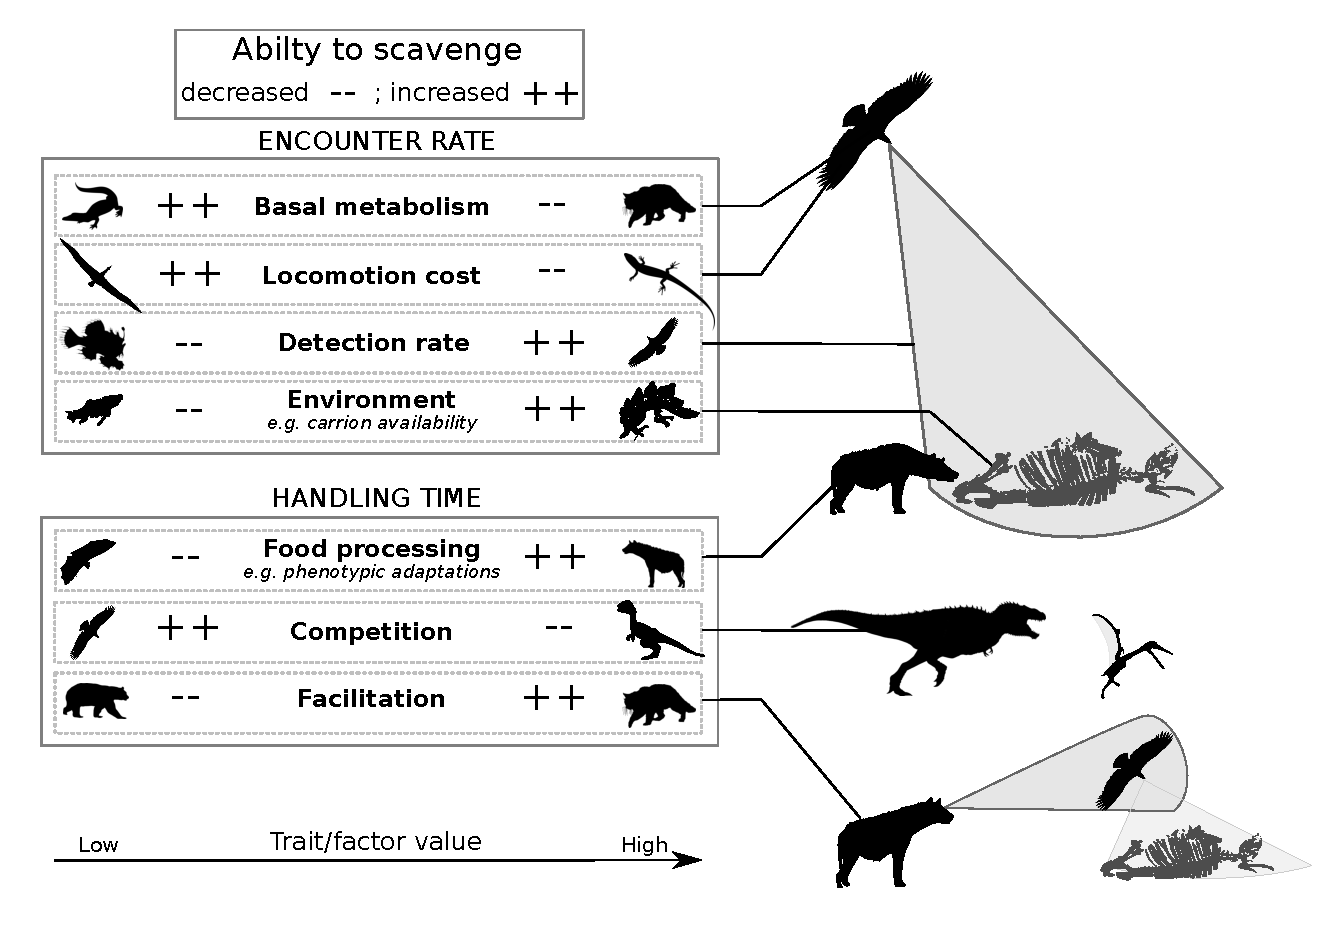
\includegraphics[width=1\textwidth]{CompositeFigure/Compositefig4.pdf}
\caption{Factors influencing the proportion of scavenging in a vertebrates' diet. Each of the traits/ factors ranges from low on the left to high on the right. A high value for a given trait can either increase scavenging propensity (+ +) or reduce it (- -), the same is true for a low value of said trait.}
\label{Summary_figure}
\end{figure}

\section{Encounter Rate}
All foraging processes depend on the encounter rate between consumer and resource. 
Locomotory speed, foraging time and detection radius all determine the encounter rate between a scavenger and the carcasses it is searching for and we would thus expect selection pressures to act on the various traits that govern these parameters.
Selection might also drive a species to reduce its metabolic requirements so that it can survive long periods between meals, or expand a species' ability to process tissues or decaying flesh that might ordinarily be discarded.
However, as we noted above, encounter rate is also determined by the productivity of the environment, and ultimately the rate at which carcasses are produced. 
\textcolor{blue}{Carcass production itself depends on factors such as predation, disease and scavenging itself. For instance, by consuming the majority of carrion, more prolific scavengers may deny a resource to their less prolific counterparts obliging the latter to hunt more, and thus, increase the amount of carrion \citep{moleon2014inter}.}

\subsection{Metabolism}
Because of the ephemeral nature of carrion \citep{devault2003scavenging,ruxton2004obligate} we expect adaptations that reduce energetic costs of maintenance to be selected for in scavengers as it would allow for longer inter-feeding periods. 
Extant reptiles possess an advantage here, in that over the course of a year their food requirements can be 30 times lower than an endotherm of equal size \citep{Nagy1621}.
\cite{devault2002scavenging} suggest this is an avenue for scavenging in snakes because they ``exhibit exceedingly low maintenance metabolisms, and most can survive on a few scant feedings per year.
It is, therefore, possible for snakes to rely largely on infrequent, less energy-rich meals."
In the same review the authors found occurrences of scavenging spread across five families of snakes and stated that this behaviour is ``far more common than currently acknowledged."\citep{devault2002scavenging}.
The same reasoning can be applied to crocodiles and their allies \citep{forrest2003evidence,moleon2015carcass}. 
\cite{carey1982temperature} found that sharks, as ectotherms, have the ability to go weeks between meals because they focus on the energy-rich sections of carcasses (see Handling Time \ref{handlingTime}). 
Endotherms have also evolved physiological mechanisms that allow them to depress their otherwise high metabolic rates at certain times e.g. vultures who do so while resting at their roost and during periods of food deprivation \citep{bahat1998nocturnal}.

\textcolor{blue}{While it is difficult to infer the metabolisms of extinct species, similarities can still also be drawn. Many ectothermic groups such as sharks and bony fish were likely to benefit from the ability to bridge long time-spans between meals such as seen in snakes. In contrast, forms such as dinosaurs \citep{grady2014evidence}, pterosuars \citep{wellnhofer1991illustrated}, some marine reptiles \citep{bernard2010regulation} and some early mammals \citep{lovegrove2016phenology} have been proposed to have possessed at least partial endothermy potentially requiring a higher intake of material in comparison to their ectothermic equivalents. However, such higher metabolic rates would also have increased the ability of such species to actively search for carrion.}
%KH: I put this section in as there is no reference in how we can use the above paragraph to infer scavenging in extinct species

\subsection{Locomotion}
\textcolor{blue}{Carrion can often be unpredictable, such as in cases where animals succumb to disease \citep{devault2003scavenging}, which means scavenging depends more on the ability to efficiently move over larger areas than does predation.}
This generally requires an efficient transfer of metabolic energy into movement which relies on the animal's anatomy and physiology as well as the medium of the environment in which the animal is moving (i.e. aerial, aquatic or terrestrial).
Perhaps the most efficient form of locomotion in vertebrates is found in flying species. 
\textcolor{blue}{Despite the energetic costs of flight, the most prolific modern, vertebrate scavengers are the old and the new world vultures.} 
While powered flight is energetically expensive, species like vultures have evolved behavioural and anatomical features to exploit air currents using their large wingspans, allowing them to soar at a cost of only around 1.5 times their metabolic rate \citep{hedenstrom1993migration,duriez2014cheap}.
By depending on thermal air flows these species can forage over vast ranges \citep{spiegel2013factors}. 
An analogous mode of locomotion is also exploited by seabirds, who use strong ocean winds to search large areas of the oceans \citep{norberg2012vertebrate,thaxter2012seabird}. 
While many species of seabird are likely primarily predators, it seems that albatrosses, who can range many hundreds of kilometres, take a substantial amount of carrion in their diet \citep{croxall1994dead}. 
This is typically in the form of squid carcases, which float on the surface, allowing the birds to readily pluck their remains out of the water \citep{croxall1994dead}. 

The groups from which these modern soaring birds arose, appeared during the Palaeocene \citep[66 - 56 Million years ago (Mya); ][]{Jetz2012, Jarvis2014} and Cretaceous \citep[145.5 - 65.5 Mya; ][]{chiappe2006early} respectively. 
However, soaring flight is likely to be far older than this with avian flight originating in the Late Jurassic (163.5 - 145 Mya) and vertebrate flight in the Late Triassic (235 - 201.3 Mya) coincident with the pterosaurs. 
Indeed, scavenging among pterosaurs has been hypothesised many times before \citep{witton2008reappraisal}. 
Certain groups of these animals could reach enormous sizes \citep[e.g. Azhdarchids with wingspans of 11 metres; ][]{witton2010size} and, notably, appear to have engaged in soaring flight \citep{witton2010size}.
It seems probable that at least some of these extinct species used soaring as a means for scavenging \citep{witton2013pterosaurs}. 

While soaring is perhaps the only viable means of locomotion that allows for scavenger to rely entirely on carrion \citep{ruxton2004obligate}, powered flight is still an efficient means of locomotion. 
Certainly, avian flight is cheaper per unit distance than either walking or running \citep{tucker1975energetic}.

We know that many extant birds exist as facultative scavengers because storks, raptors and corvids all take substantial quantities of carrion in their diet \textcolor{blue}{\citep{mateo2015regional}}. 
Similarly we would expect that extinct species would also scavenge in a similar fashion depending on the efficiency of their flight. 
For example, early birds such as \textit{Archaeopteryx} are predicted to have been poor, relatively inefficient fliers \citep{nudds2010narrow} and so ill-suited to finding carrion. 
The importance of efficient flying over large areas may explain the lack of scavenging behaviour in bats as they are generally nocturnal, a time when they would receive no aid from convective air currents \citep{norberg2012vertebrate}. 

Similar to aerial species, aquatic scavengers have a locomotory benefit because water is a medium that is conducive to low-cost movement \citep{tucker1975energetic,williams1999evolution}.
This has led some researchers to argue for the likelihood of an obligate scavenging fish \citep{ruxton2004energetic,ruxton2005searching}. 

Sharks are one likely candidate for general scavenging behaviors as their locomotion, which depends on large pectoral fins to generate lift as they swim, resembles that of the large soaring fliers.
Many shark species have large foraging ranges \citep[e.g. the great white sharks \textit{Carcharodon carcharias};][]{bruce2006movements} and it seems reasonable that they would use oceanographic currents to further reduce movement costs \citep{ruxton2004energetic}.
In fact, facultative scavenging is seen in many selachian groups, including species of extant sharks like white sharks \citep[known to feed on whale carcasses;][]{fallows2013white}, Greenland sharks \citep[feeding on seals;][]{watanabe2012slowest}, and sixgill sharks \citep{anderson2016impact}. 
There is evidence too of scavenging in extinct species, where shark teeth have been found in the remains of dinosaurs, mosasaurs and Pliocene mysticete whales \citep[5.3 - 3.6 Mya; ][]{schwimmer1997scavenging,ehret2009caught}. 

Interestingly, however, style of swimming in fishes does not significantly affect the cost of movement \citep{williams1999evolution}. Hence, it is likely that many aquatic species with large ranges will encounter scavenging opportunities. 
% It is perhaps jaw morphology that is more likely to define which species can avail of carcasses.

We might expect then that by combining an aquatic environment and an endothermic metabolism marine mammals would especially prosper as scavengers. 
Fossil pinnipeds and cetaceans from 60 Mya have transitional features indicative of their evolutionary trajectory to fully aquatic species \citep{williams1999evolution}.  
But despite their movement away from land their energetic savings were negligible because the \textit{total} cost incurred by a swimming marine mammal is high \citep{williams1999evolution}. 
Indeed, the total energetic cost is similar to an equivalent terrestrial or aerial mammal \citep{williams1999evolution}.
This underscores the trade offs between the benefits of endothermy in terms of activity periods and the costs of maintaining such an energetically expensive system. 
That said, aquatic endotherms have and do scavenge. 
For instance, early whales such as \textit{Basilosaurus} (38 - 36.5 Mya) seem to have fit into the same niche as killer whales (\textit{Orcinus orca}) and we have some evidence for scavenging in both \citep{fahlke2012bite,Whitehead415}.

Terrestrial environments are the most energetically costly in which to move \citep{tucker1975energetic}. 
Unlike aerial and aquatic environments, support must be provided through the animal's posture. 
The early transition from a sprawling gait, seen in early tetrapods, to the more erect posture of synapsids and later dinosaurs and mammals, has often been supposed as conferring a huge advantage to the latter groups \citep{sullivan2015posture}.
The purported advantages include benefits in terms of speed, efficiency, muscle effort and manoeuvrability \citep{sullivan2015posture}.
Clearly, for a scavenger, an ability to efficiently cover an area at a high speed would increase the encounter rate with carrion. 
Despite being intuitive, \cite{sullivan2015posture} states most of the hypotheses in favour of this idea remain to be tested in the context of archosaur evolution. 
One noted consequence of a sprawling gait is the phenomenon known as Carrier's constraint such that the animal can't move and undergo coastal ventilation at the same time because the lateral movements impedes its lungs \citep{carrier1987evolution}. 
The evolution of an upright posture has been offered as one of the primary mechanisms that allowed early archosaurs to overcome this constraint \citep{uriona2008recruitment}. 

Whatever the case, it is with the evolution of endothermy in the therapsid-mammal lineage \citep{clarke2010temperature} that terrestrial vertebrates would have gained the ability to range more widely, a vital component in seeking out carrion.
Modern endothermic mammals can sustain longer periods of energetically expensive activity \citep{bennett1979endothermy} resulting in larger foraging ranges. 
Today, terrestrial scavenging in mammals is probably best known in the \textcolor{blue}{African Savannah context where hyenas and lions can all take sizeable proportions of carrion in their diet \citep{pereira2014facultative,periquet2015lion}.}
In the spotted hyena (\textit{Crocuta crocuta}), striped hyena (\textit{Hyaena hyaena}) and brown hyena (\textit{Hyaena brunnea}) it can be over 90\% \citep{jones2015african}.
\textcolor{blue}{Most, if not all, vertebrate terrestrial carnivores take carrion to some extent \citep{devault2003scavenging,beasley2015vertebrates,pereira2014facultative}}.
\textcolor{blue}{The particular ability of hyenas to subsist on high proportions of carrion means we can use them as examples of efficient terrestrial scavengers to compare with other forms \citep{periquet2015lion}}. 
In terms of locomotion, they employ a characteristic ``rocking horse gait''  which allows them to cover great distances efficiently, loping at 10 km/hr \citep{mills1989comparative,jones2015african}. 
Such long-distance travel is apparent \textcolor{blue}{in many other cursorial predators \citep{pennycuick1995radius,janis2014forelimb,pereira2014facultative}. 
In contrast, big cats rely on ambush \citep{pennycuick1995radius,pereira2014facultative}. 
This difference means ambush predators tend to be more obligate hunters \citep{pereira2014facultative}.} 
These insights allow us to compare extant terrestrial species to their prehistoric forebears given the dominance of mammalian carnviores since the Eocene (56-33.9 Mya) where the order split into the Caniforma and Feliforma \citep{van1987skeletal}.
To take one example, \cite{anyonge1996locomotor} found that \textit{Nimravides}, a genus of sabretooth cat from the Miocence (10.3 - 5.3 Mya), were likely to have been ambush predators which would argue against them taking a lot of carrion. 

Of course, terrestrial animals can also move bipedally. 
Although the evolution of bipedal movement was significant in that it freed up the forelimbs for other purposes (e.g. climbing, tool-use, wing development etc.) it does not differ radically in cost from quadrupedal locomotion (\cite{williams1999evolution}, \textcolor{blue}{and references therein}). 
For instance, \cite{alexander2004bipedal} shows that, in the case of humans, we are more economical than predicted while walking and less so while running according to predicted costs of terrestrial movement calculated by allometric scaling relationships.
Our locomotory efficiency has fed into the question of where our ancestors placed on the hunter-scavenger axis during the Plio-Pleistocene, which has been a matter of debate for years \citep{capaldo1995skeletal,dominguez2002hunting}.
\cite{ruxton2013endurance} added to this debate with their argument that long distance endurance running \textcolor{blue}{was not an important feature of hominin scavenging but was instead used by humans for hunting prey by chasing them to exhaustion over large distances.
Even when considering the use of weapons and social foraging, the authors argue that the high cost of running long distances would render it an unattractive foraging strategy for scavenging.}

Aside from humans and our allies, the best-known terrestrial bipeds are the dinosaurs and unsurprisingly, given their enduring appeal, the prevalence of scavenging has been extensively explored in the carnivorous theropods.
These were the dominant terrestrial carnivores for most of the Mesozoic Era (252.17 - 66 Mya) and ranged from the chicken-sized to the whale-sized, all of which were bipedal.
While the locomotory ability of theropods has been debated since their first inception, more recent studies have reconstructed them as relatively mobile animals \citep{pontzer2009biomechanics}. 
Despite some suggestions that larger species may have had some advantage in scavenging, partially due to the ability to search large areas \citep{ruxton2003could}, more recent work has shown that the energetic demands of locomotion in such large forms meant scavenging was likely more prevalent in mid-sized theropods of approximately half a tonne \citep{kane2016body}.

\subsection{\textcolor{blue}{Sensory} Detection}

As predicted by the importance of an increased encounter rate, known scavengers have evolved well-developed senses, with the visual and olfactory sensory systems most often associated with scavenging behavior. 
This is perhaps no surprise because sensory systems that rely on detecting signals associated with living animals, such as audioception, electroreception, thermoreception and echolocation will be limited in their ability to detect an already dead animal.

Apart from the basic capacity of these senses to detect carrion, how they function in different environments is also important. 
In the simplest case, the search space is a two dimensional plane \citep{pawar2012dimensionality}. 
If the scavenger itself is searching on the plane, as is so for terrestrial species, the detection range is simply defined by the radius of their sensory organs.
Consequently, the ability to detect carrion can be seriously restricted for visually reliant, terrestrial species. 
They may overcome this restriction however, by using olfaction, which is less affected by the relief of the land.
For example, hyenas have the ability to smell a rotting carcass 4 km away \citep{mills1989comparative}, which exceeds the 500 m range deemed necessary by \cite{ruxton2004obligate} to be able to survive as a scavenger. 

Indeed, the olfactory senses of many extant (and in all probability extinct) carnivores meet this required distance, making scavenging feasible for most terrestrial carnivores \citep{farlow1994speculations,mech2010wolves}. 
Among extinct species in particular, we can use the ratio of olfactory bulb to brain size to infer a preference for olfactory foraging \citep{zelenitsky2011evolution}.
This approach was used by \cite{zelenitsky2011evolution} to hypothesise such a mode for the theropod dinosaur \textit{Bambiraptor} and by \cite{witmer2009new} for tyrannosaurs.
The flying pterosaurs however, had tiny olfactory bulbs indicating this sense was not relied on \citep{witton2013pterosaurs}.

Species capable of flight have added an extra spatial dimension (i.e. the vertical component) to their sensory environment over land animals.
This allows them to look down on a landscape where they are unencumbered by obstacles that would obstruct the view of a terrestrial scavenger.
In this way they are effectively cheating the 2D system by gaining a bird's eye view which has has obvious benefits in detecting carrion.
Certainly, vultures are known to have impressive visual acuity, with one estimate indicating lappet-faced vultures (\textit{Torgos tracheliotus}) are capable of detecting a 2 metre carcass over 10 km away \citep{spiegel2013factors}.
Eagles too are known to have highly developed vision \citep{reymond1985spatial}.
The flying pterosaurs also convergently evolved large orbits and optic lobes \citep{witton2013pterosaurs}. 
It follows that the evolution of flight allowed aerial animals to detect far more carrion than their terrestrial counterparts through vision \citep{AR:AR22815}.

The terrestrial-olfaction, aerial-visual divide is not total though.
Terrestrial species like hyenas and hominins exploit the efficiency of birds by looking to the skies for groups of vultures to follow to carrion \citep{jones2015african,ruxton2013endurance}. 
And many birds, e.g. turkey vultures (\textit{Cathartes aura}), have well-developed olfactory systems \citep{AR:AR22815} which they use to forage in heavily forested areas where vision is limited \citep{houston1986olfaction}. 

Although aquatic species also have a vertical component to their environment, they must contend with low-light levels where visual detection distances are far lower ($<$ 100 m) than they would be for air.
As such, aquatic animals detect resources through chemo- and mechanoreception more so than through vision \citep{ruxton2004energetic}.
This is particularly relevant to sharks and aquatic snakes who are deemed as having the most suitable physiology for scavenging.
A hypothesis put forth by \cite{sazima1990necrofagia} argued that chemical gradients in water would allow for a relatively easier detection of carrion by snakes.
This gained some support from \cite{devault2002scavenging}, who found a preponderance of aquatic snake species in their review of this behaviour.
Smell seems to be the primary means of carcass detection in sharks as well. 
\cite{fallows2013white} found that wind speed determined the number of sharks feeding at whale carcasses due to chemical stimului from the carcasses being propogated through the water by the wind, indicating they were dependent on detecting the odours from the decaying whales.

\subsection{Carcass Availability}
\subsubsection{\textcolor{blue}{Abiotic effects}}
The environmental influence on \textcolor{blue}{carcass} availability is an aspect that greatly affects encounter rate. %but is invisible to the selective forces acting on the scavenger. 
Aspects including, primary productivity, relief, and temperature will all affect scavenging tendency. 

\cite{ruxton2004obligate} suggest an historic ecosystem with a productivity similar to the Serengeti could have supported an \textit{obligate} mammalian or reptilian terrestrial scavenger.
Indeed, in systems that were dominated by large ectothermic or mesothermic herbivore vertebrates, the same primary productivity would have supported a greater biomass, due to the scaling of mass with metabolic rate \citep{mcnab2009resources}.
The upshot of this may have been a higher biomass of herbivores dying and offering scavenging opportunities (although these larger species may have also lived longer).

In fact, scavenging behaviour may have evolved on land as soon as the first terrestrial tetrapods emerged.
Some of the earlier tetrapods tracks dating back to the early Middle Devonian (393.3 - 387.7 Mya) were found in intertidal environments \citep{Niedzwiedzki2009}.
These environments are isolated from marine systems twice a day leaving potential carrion unexploited by marine vertebrates.
\cite{Niedzwiedzki2009} suggest that these environments ``would thus have allowed marine ancestors of tetrapods gradually to acquire terrestrial competence while accessing a new and essentially untouched resource.''

\textcolor{blue}{The physical differences between water and air mean carcass availability is radically different between these environments \citep{beasley2012carrion}. 
For one, carcasses get moved around by water which results in a more diffuse signal being produced for would-be scavengers.
Carcasses also tend to sink in water where they are no longer accessible to pelagic scavengers \citep{beasley2012carrion}. 
\textcolor{blue}{Research has shown that an animal need only travel 36 km to encounter a fresh whale carcass \citep{smith2003ecology}.} 
The phenomenon of occasional bounties of carrion in the form of these whale falls has led some researchers to investigate if a scavenger could survive by seeking out these remains exclusively.}
\cite{ruxton2005searching} argued that although this is energetically feasible it's ecologically unlikely.
Any animal that could find such whale carcasses is unlikely to have ignored other types of carrion. \\
Although no aquatic species have ever exceeded the size of whales, some enormous animals have evolved in this environment before the evolution of cetaceans, including \textit{Leedsichthys}, a bony fish from the Middle Jurassic (174.1 - 163.5 Mya) and the aquatic Mesozoic reptiles, the plesiosaurs, pliosaurs and ichtyosaurs, that could all exceed 15 metres in length \citep{ruxton2011zoology,danise2014ecological}.
So, despite being unlikely, the energetic feasibility of a marine scavenger that specialises on large carcasses has a long history.

% KH: Is there an estimate of how much of the fishes diet can be made up from this type of scavenging?

Perhaps the greatest environmental driver of scavenging tendency is that of temperature which has a significant bearing on the availability, predictability and persistence of carrion.
We know from the geological record that the Earth has undergone radical fluctuations in temperature over time.
\textcolor{blue}{On land, there are a wide variety of vegetation types, from thickly forested areas to open grassland and the extent of this vegetation changes with season.}
%All of these factors influence the availabiltiy of carrion.  
%Moreover, oceanic productivity is also impacted by climactic conditions. 
%KH: I would delete the last two lines of this paragraph and merge it with the next one
To illustrate the point, a 10$^{\circ}$C increase in ambient temperature can double carcass decomposition rates \citep{parmenter2009carrion} and geological evidence indicates that the Mesozoic Earth was on average at least 6 $^{\circ}$C warmer than now \citep{sellwood2006mesozoic}.
In terms of specific habitats, it has been shown that decomposition is greater in warm and moist areas versus more xeric ones \citep{beasley2015vertebrates}.
The impacts these can have on scavengers have been empirically supported e.g. \cite{beasley2015vertebrates} who point to a series of studies showing how microbes and invertebrates benefit at higher temperatures to the detriment of vertebrate scavengers such that ``above 20$^{\circ}$C vertebrates were able to detect and consume only 19\% of small-mammal carcasses, whereas at temperatures below 18$^{\circ}$C, vertebrates consumed 49\% of carcasses".
\textcolor{blue}{
Spikes in temperature can result in severe droughts causing mass mortality events which result in relatively predictable peaks in carrion availability \citep{kendall2014african}.%In savannah, dense vegetation can prevent vultures from landing to a carcass because they will be unable to take off again \citep{bamford2009effect}.
%KH: This is a biotic interaction so I would either remove it or move it somewhere else. 
The Earth has also undergone a series of ice ages of various spatio-temporal extent \citep{diedrich2012cave} and modern terrestrial settings that experience sub-zero conditions can act as a microcosm to show the effect extreme cold can have on scavenging.
Notably, freezing carcasses can become too hard to consume by most vertebrate carnviores \citep{selva2003scavenging}.}

\subsubsection{\textcolor{blue}{Biotic effects}}
Foragers do not exist in isolation and we know from field observations that scavengers can scrounge on the discoveries of other carnivores. 
This sort of facilitation occurs across a range of scavengers, in the air and on the ground \citep{KaneVul,jones2015african}. 

In flight, birds are able to gather a wealth of information from other foragers, be they conspecifics or otherwise \textcolor{blue}{\citep{jackson2008effect,KaneVul,moleon2014inter}}.
% These interactions are properly three dimensional in the sense of \cite{pawar2012dimensionality} because both producer and scrounger are in the air \citep{dall2005information}. 
Again, returning to vultures, the genus \textit{Gyps} consists of highly social and colonially nesting species \citep{fernandez2015density}.
These behaviours allow them to forage far more efficiently because one bird can scrounge information on the location of food from another successful forager \textcolor{blue}{\citep{cortes2014bird}}.
Information transfer of this kind is typically inadvertent and as a consequence no complex social interactions are required, simply the ability to recognise a successful forager.
\textcolor{blue}{Thus, given pterosaurs seem to have cohabited in large numbers \citep{witton2013pterosaurs}, and the theoretical benefits this can have for social foraging in birds \citep{jackson2011evolutionary}, it seems probable that scrounging behaviours were seen in the flying pterosaurs as well.} 

\textcolor{blue}{This type of facilitation then increases the encounter rate of the facilitated species and can increase the population size of the latter \citep{moleon2014inter}. 
This higher population of predators may take more prey and so produce more carcasses.
Conversely, by feeding on carcasses, predators may hunt less because they are sated by carrion, ultimately reducing predation risk on their prey base \citep{moleon2014inter}.} 

\textcolor{blue}{Modern scavenging assemblages are known to be influenced by carcass size \citep{moleon2015carcass}. 
Larger carcasses tend to last longer and also present a more conspicuous target for a foraging scavenger which results in more species attending them \citep{moleon2015carcass}.
This will have had implications for extinct assemblages because body size distributions vary across different environments but also across time. 
\cite{10.1371/journal.pone.0051925} showed Mesozoic faunal distributions may have been skewed towards larger species even when fossil biases are taken into account. 
Similarly, the megafauna of the Pleistocene \citep{doughty2013legacy} would have produced large carcasses. 
As a result, the scavenger assemblages during this era would have been particularly diverse.}

\section{Handling Time}
\label{handlingTime}
Since the food a scavenger depends upon is not dispatched directly, often the most easily accessible and choicest components of the carcass will be missing owing to the activity of predators and other scavengers, or, if present, will be subject to decay as well as competition.
So being able to overcome competitors and maximise the nutrient gain from the remnants are all essential parts of carcass handling time. 

\subsection{Competition}
Large body size has substantial advantages in agonistic interactions \textcolor{blue}{\citep{ruxton2004obligate,moleon2014inter,pereira2014facultative}}. 
For instance, lions can acquire much of their carrion through kleptoparasitism of hyena kills \textcolor{blue}{\citep{trinkel2005competitive,pereira2014facultative,periquet2015lion}}. 
This line of reasoning suggests that some theropod dinosaurs, who could get up to 15 tonnes, would have easily monopolised a carcass \citep{weishampel2004dinosauria} provided they could find them efficiently \citep{kane2016body}. 

We would expect this trait to be selected for even in the case of weight-constrained, scavenging fliers.
This is true for \textcolor{blue}{many vultures and other major avian scavengers such as albatrosses who can have body masses in excess of} 10 kg and represent some of the heaviest bird species capable of flight \citep{weimerskirch1992reproductive,ferguson2001raptors,donazar2002effects}.
Indeed, such is the competitive advantage held by vultures over other facultative scavenging birds that temporal niche partitioning at the carcass has evolved \textcolor{blue}{\citep{kendall2013alternative,KaneVul,moreno2016behavioral}}. 
Additionally, many pterosaurs were far bigger again, with estimated body masses of over 200 kg in the Azhdarchids \citep{witton2010size}.
Although \cite{witton2008reappraisal} argued that neck inflexibility and straight, rather than hooked jaw morphology points against Azhdarchids being \textcolor{blue}{as well adapated as vultures} to scavenging, their terrestrial proficiency indicates they would have been comfortable foraging on the ground.
Extant Marabou Storks (\textit{Leptoptilos crumeniferus}) have a comparable morphology and are noted facultative scavengers \citep{monadjem2012survival} so it is reasonable to believe that these pterosaurs behaved similarly.

By contrast, extant bats seem poorly equipped to deal with competitors. 
Their poor terrestrial ability, small size and cost of movement on the ground would count against them while attempting to fend off other species at a carcass \citep{riskin2006terrestrial,voigt2012terrestrial}.

Smaller species can compensate for a lack of individual body size by weight of numbers in competitive interactions. 
This is true for a host of notable scavengers, such as vultures, early hominins and hyenas, who can and could dominate larger competitors provided they substantially outnumber(ed) them \citep{KaneVul,trinkel2005competitive,ruxton2013endurance}. 

Direct confrontation can be circumvented by certain behavioural adaptations. 
The evolution of nocturnal behaviour in some mammals, for instance, has been put forth as an adaptation to reduce competition with the exclusively diurnal vultures as well as with other larger predators \citep{gittleman2013carnivore,moleon2014inter,pereira2014facultative}. 
In areas absent of vultures such as the Arctic, terrestrial carnivores like bears and wolves take more carrion \citep{devault2003scavenging}
Thus, in the Palaeozoic, the absence of flying vertebrate competitors may have permitted terrestrial forms to take in a higher proportion of carrion in their diet.

In addition to fending off other vertebrates, scavengers also have to contend with competition from \textcolor{blue}{invertebrates and micro-organisms, the latter of which may require a specialised physiology.} 
Although the findings of \cite{shivik2006vultures} that ``evolutionary pressures favor detection maximizers relative to toxification minimizers in competitive interactions for carcasses." appear sound, the fact remains that overcoming micro-organism toxins is still a beneficial adaptation to any scavenger. 
Avian scavengers have evolved incredibly acidic stomachs that allow them to consume and process putrefied flesh with no ill effects \citep{houston1975digestive,roggenbuck2014microbiome}. 
This adaptation is not restricted to vultures though, \cite{gremillet2012vultures} showed wandering albatrosses (\textit{Diomedea exulans}; so-called ``vultures of the seas'') had an average stomach pH of 1.5, which enables them to consume fisheries discards and squid carcasses. 
There is also evidence of selection for ``toxification minimizers'' beyond birds among the ectotherms.
From our earlier arguments we know that ecthotherms are limited in their ability to find carrion as quickly as endotherms. 
These later arrivers would thus benefit especially from well-developed detoxifying apparatus. 
\cite{shivik2006vultures} suggests that ``specialized oral structures in snakes may have evolved under pressures associated with scavenging."
Moreover, some researchers have charted an evolutionary course from basal fossorial snakes to modern terrestrial species by way of a scavenging intermediate \citep{bauchot2006snakes}. However, snake venom is primary associated with predation in extant species suggesting that if venom played such a role aiding digestion of discovered carcasses in extinct species it is no longer its main function \citep{casewell2013complex}.
\textcolor{blue}{In water, by contrast, competition with micro-organisms is significantly reduced because of the high pressures and low temperatures \citep{beasley2012carrion}.}

\textcolor{blue}{\subsection{Facilitation}
In contrast to competitive interactions, there are facilitatory processes at play between vertebrate scavengers that can benefit the facilitated species. 
Rather than there being a random assortment of species at a carcass, scavenging assemblages tend to be nested \citep{selva2007nested}. 
This means the species that feed on the majority of carcasses, for example vultures, are a subset of a larger community which comprises hyenas, jackals, raptors etc. \citep{sebastian2016nested}. 
We noted above that this often results in an increased encounter rate but it can also reduce handling time for the species that follow. 
% In extant systems these interactions can reduce handling times for the facilitated species. 
Some examples of reduced handling time include vultures, hyenas and wolves opening the tough hides of ungulate carcasses that would otherwise be inaccessible to corvids and smaller mammalian carnivores \citep{selva2003scavenging,moleon2015carcass}. 
Unfortunately these interactions are particularly difficult to detect in extinct species.}



\subsection{Food Processing}
Another vital component of carrion handling time is the ability to maximise the energy gain from the remains while reducing the energetics of doing so. 
At whale carcases, white and blue sharks are known to preferentially feed on the blubber layer \citep{long1996sharks}. 
Blubber is an energy rich portion of the carcass that can allow a shark to survive for 1.5 months on 30 kg of the material \citep{carey1982temperature}. 
On land many scavengers utilize late-stage carcass material that is less subject to decomposition and may be unavailable to other competitors, for example bone.
Osteophagy is known across a range of terrestrial carnivores and given that some fat-rich mammalian bones have an energy density (6.7 kJ/g) comparable with that of muscle tissue, it makes skeletal remains an enticing resource \citep{brown1989study}.
\textcolor{blue}{Within mammals,} this ability reached its zenith among hyenas with the evolution of the estimated 110 kg \textit{Pachycrocuta brevirostris} during the Pliocene \citep[3.6 - 2.58 Mya; ][]{palmqvist2011giant}.
Indeed, their extinction has been blamed on the decline of sabretooth cats (Machairodontinae), \textcolor{blue}{because} the unique skull morphology of the latter meant they would leave a large amount of food on a carcass for would-be scavengers (\citealt{palmqvist2011giant}; \textcolor{blue}{note, however that the inability of these cats to deal with bone may be overstated; \citealt{binder2010comparison}}). 
Earlier in the evolution of mammals, the bone-crushing dogs that evolved during the Oligocene (Borophaginae; 33.9 - 23.03 Mya) have also been compared to hyenas in terms of their feeding ecology \citep{van2003chapter,martin2016pursuit}.

In Mesozoic systems some large theropod dinosaurs had a morphology indicative of an ability to process bone \citep[e.g. the robust skull and dentition of \textit{Tyrannosaurus rex;}][]{hone2010feeding}.
There is direct evidence that \textit{T. rex} did this in the form of distinctive wear marks on its tooth apices \citep{farlow1994wear,schubert2005wear} and the presence of bone fragments in its coprolites \citep{chin1998king}.
The animal also had an enormous bite force, with one estimate putting it at 57000 Newtons \citep{bates2012estimating} which would have been powerful enough to break open skeletons \citep{rayfield2001cranial}.
Osteophagy may have been even more viable during the Mesozoic era as well because of the skewed body mass distribution of herbivores towards larger sizes \citep{10.1371/journal.pone.0051925}.
When we couple this with the fact that skeletal mass scales greater than linearly with body mass \citep{prange1979scaling} there would have been a lot of bone material to consume in the environment provided an animal had the biology to process it \citep{chure1997one}.

Despite not having the anatomical ability to break open bone, the bearded vulture (\textit{Gypaetus barbatus}) has evolved a technique whereby it drops long bones from a height, splintering them on the rocks below which allows them to feed \citep{margalida2008bearded}. 
Similarly, early hominins developed the ability to craft tools for breaking open bones \citep{ARCM:ARCM12084}.
A recent study investigating potential scavenging opportunities for hominins in Kenya found that, in addition to skeletal material, there is a substantial amount of scavengeable meat left on predated remains; sufficient to sustain the requirements of an adult male \textit{Homo erectus} \citep{pobiner2015new}.
In some historical hominin-inhabited areas there were \textcolor{blue}{higher populations of felids compared to hyenids.}
Again, this is significant because hyenas are likely to have left far less flesh on a carcass than a felid such as a sabretooth, enabling contemporaneous hominins to benefit \citep{pobiner2015new}.
The use of tools and the cooperative nature of hominins meant they could likely get a substantial part of their energetic requirements through scavenging depending on their environment \citep{moleon2014humans}.

On the ground, and despite the advantages of social resource defence, the competitive ability of even the largest flying bird is radically diminished in their interactions with mammalian competitors, and as such they tend to consume carrion rapidly. 
\cite{houston1974role} observed a group of \textit{Gyps} vultures consuming all of the soft tissue from a 50 kg Grant’s gazelle (\textit{Nanger granti}) in eight minutes. 
Their serrated tongues and hooked bills enable them to achieve this feat \citep{houston1975digestive}. 
Aside from raptors, the specialised beaks of many modern bird lineages tends to hinder their ability to eat meat which is in contrast to the first lineages that did not have this feature \citep{martyniuk2012field}. 
As \cite{martyniuk2012field} notes, \textcolor{blue}{this skull morphology of early birds indicates} they were predominantly carnivorous, implying scavenging was a live opportunity compared to many of their descendants. 
Among the pterosaurs, \cite{witton2013pterosaurs} makes the case that the istiodactyl pterosaurs were the most likely scavengers of this group based on their potential handling time. 
Their skull morphologies are indicative of animals that were suited to removing large amounts of flesh from an immobile foodstuff \citep{witton2013pterosaurs}. 

Again, we can draw a comparison with species that are lacking in these features. 
\textcolor{blue}{Despite readily eating carrion in captivity, cheetahs (\textit{Acinonyx jubatus}) and African Wild Dogs (\textit{Lycaon pictus}) rarely do so in the wild because they are subordinate to many of the mammalian competitors they coexist with \citep{pereira2014facultative}.} 
Extant bats are poorly equipped when it comes to feeding on carrion; the larger forms are typically frugivores and therefore lack the adaptations for digesting meat, while the smaller carnivorous bats are mainly found in the microbats, which are insectivorous \citep{aguirre2003implications}.   
That said, Necromantis (“death-eater”), a large bat from the middle to late Eocene (56 - 33.9 Mya) had a robust cranio-mandibular morphology, and is a likely candidate for an extinct scavenging bat \citep{Weithofer_Necromantis_1887,Hand_Necromantis_2012}.

%\begin{figure}[!htbp]
%\centering
%   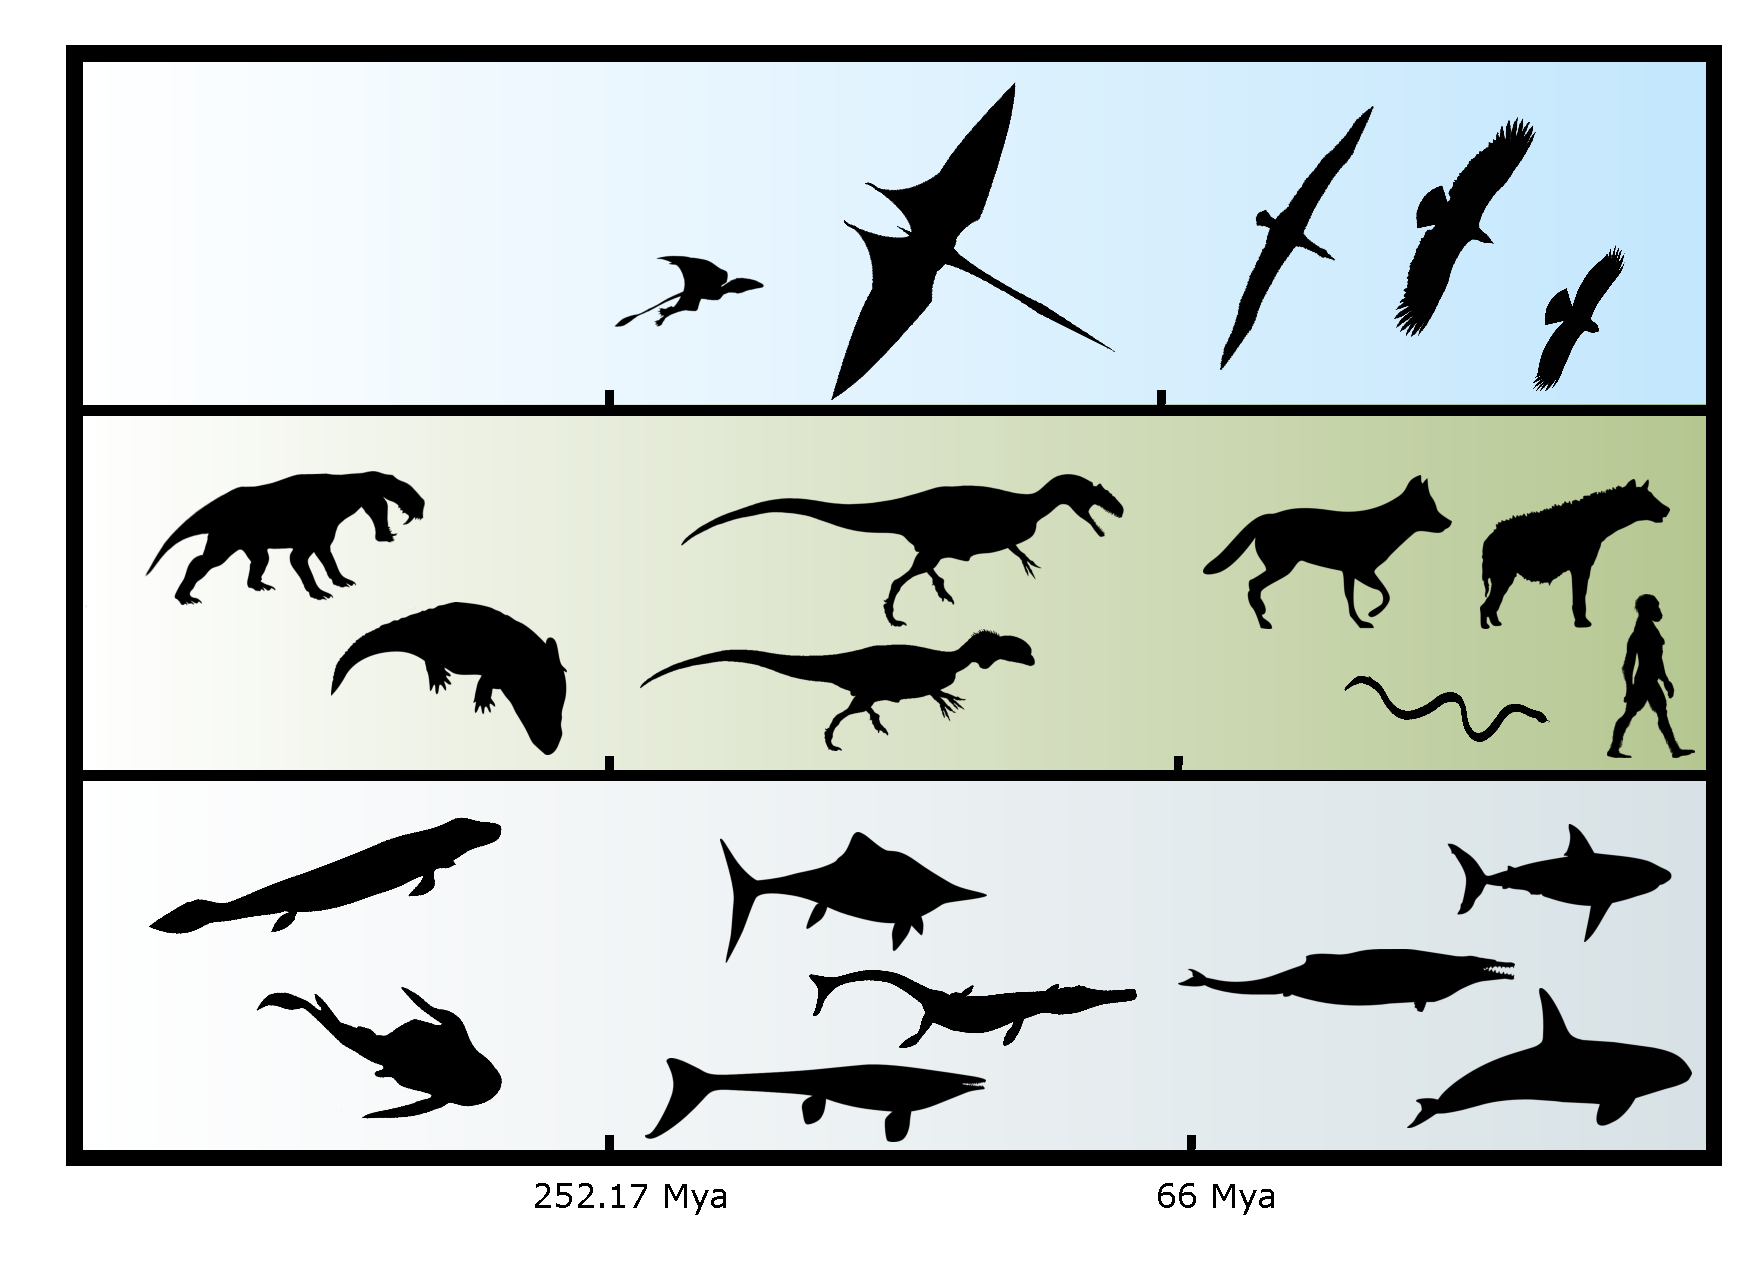
\includegraphics[width=1\textwidth]{timeline_figure/timeLine.pdf}
%\caption{The diversity of scavengers through time. Each species has either direct evidence for it being a scavenger or would be positioned high up on our scavenging scale. The three lines represent the three different environments (from top to bottom: aerial, terrestrial and aquatic). Time is represented on the horizontal axis with each third representing respectively the Paleozoic (541 - 252 Mya), the Mesozoic (252 - 66 Mya) and the Cenozoic (66 Mya to the present).}
%\label{Timeline}
%\end{figure}

\section*{Conclusion}
As is often the case in science, the present provides the key to the past.
The animals of today, while often different (sometimes radically so) to their ancestors, can be used to make informed comparisons to extinct species. 
We have used this \textcolor{blue}{approach} to give insight into the drivers of scavenging across vertebrates through time.
In common with any other forager be they grazer, browser or predator, scavengers past and present have had to balance their energetic costs with the gains of food. 
The main factors we considered namely, encounter rate, handling time and prey availability can be used to create a scale of scavenging whereupon any species can be placed in order \textcolor{blue}{to predict the qualitative importance} of carrion in it diet.
We hope this approach will be useful in the effort to explore this most understudied of feeding ecologies. 

\section*{Appendix}
Scaling relationships for sustainable travel speed are 1.15 $\times$ body mass (kg) \textsuperscript{0.12} and 0.23 $\times$ body mass (kg) \textsuperscript{0.12} for mammals and reptiles respectively \citep{ruxton2004obligate}.
These are fed into the foraging model $\sfrac{\frac{\text{duration} \times \text{speed}}{2}}{1000}$ \citep{Enstipp2006Energetics}.

\section*{Acknowledgments}
Thanks to Natalie Cooper for highlighting the potential for this review, and to Ara Monadjem and Deirdre McClean for their comments on the manuscript. We also thank Marcos Moleón and two other anonymous reviewers for very perceptive and helpful feedback on a previous version. 

\newpage

\bibliography{bibfile}

\end{document}






% Modern scavenging assemblages can be influenced by carcass size \citep{moleon2015carcass}. 
% Larger carcasses tend to last longer and also present a more conspicuous target for a foraging scavenger which results in more species attending them \citep{moleon2015carcass}.
% This will have had implications for extinct assemblages because body size distributions vary across different environments but also across time. 
% \cite{10.1371/journal.pone.0051925} showed Mesozoic faunal distributions may have been skewed towards larger species even when fossil biases are taken into account. 
% If this pattern is real then the scavenger assemblages during this era would have been particularly diverse. 

% As well as competitive interactions, there are also facilitatory processes at play between vertebrate scavengers that can reduce handling time. 
% Rather than there being a random assortment of species at a carcass, scavenging assemblages tend to be nested \citep{selva2007nested}. 
% This means the species that feed on the majority of carcasses, for example vultures, are a subset of a larger community which comprises hyenas, jackals, raptors etc. \citep{sebastian2016nested}. 
% In extant systems these interactions can reduce handling times for the facilitated species. 
% Some examples include vultures, hyenas and wolves opening the tough hides of ungulate carcasses that would otherwise be inaccessible to corvids and smaller mammalian carnivores \citep{selva2003scavenging,moleon2015carcass}. 
% The availability of carcasses can be indirectly influenced by the action of scavengers. 
% Through facilitation e.g. local enhancement, vultures may increase the amount of carrion mammalian carnivores feed on thus increasing their population size \citep{moleon2014inter}. 
% This higher population of predators will take more prey and so produce more carcasses. Conversely, by feeding on carcasses, predators may hunt less because they are sated by carrion, ultimately reducing predation risk on their prey base \citep{moleon2014inter}. 



%Carcass size shapes the structure and functioning of an African scavenging assemblage
%Moleon et al
%We found strong evidence indicating that carcass size is a major factor governing the associated scavenger assemblage. Scavenger species richness per carcass and carcass consumption time and rate increased with carcass size, while carcass detection time and percentage of carrion biomass consumed were negatively related to carcass size. 
%During the dry season, less vegetation cover might also favor the detection of carrion by scavengers, especially mammals (Ruzicka and Conover 2012).
%The mean number of scavenger species exploiting a particular carcass increased with carcass size, probably because the longer temporal availability and higher conspicuousness of larger carcasses (DeVault et al. 2004) allowed more species to aggregate.
%This suggests that hyenas were involved in some interactions that enhance community structure, such as carcass signaling and tearing open of thick-skinned animals (Moleón et al. 2014a). 
